\begin{frame}
{Image analysis tasks}

Let $I:\mathbb{Z}^2\rightarrow[0,1]^3$ a colored image.\\[1em]

\begin{minipage}[t][0.25\textheight][t]{0.5\textwidth}
\center
Segmentation\\

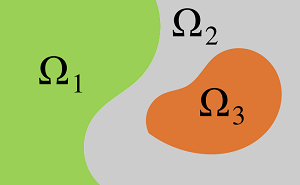
\includegraphics[scale=0.5]{figures/motivation/image-analysis/segmentation-stylised.png}
\end{minipage}%
\begin{minipage}[t][0.25\textheight][t]{0.5\textwidth}
\center
Inpainting\\


\includegraphics[scale=0.5]{figures/motivation/image-analysis/inpainting-stylised.png}
\end{minipage}%
%
\begin{align*}
 \argmin_{I^\star} &= \min_{I} Data(I) + Reg(I).
\end{align*}
%
Common geometric regularizers: perimeter, area.

\end{frame}